% Nome do capítulo

\chapter{PondiônsTracker}
% Label para referenciar
\label{cap4}

% Diminuir espaçamento entre título e texto
\vspace{-1.9cm}

% Texto do capítulo
In this Chapter, we present \textit{PondiônsTracker}\footnote{Available at \url{https://github.com/Pongelupe/PondionsTracker/}}, 
which is a framework to enrich
GTFS data with real-time data enabling { \em collecting } and { \em integrating }. 
The name \textit{PondiônsTracker} is a small gag from the sonority of the expression{ \em bus stop}
when pronounced in Portuguese with the accent from Minas Gerais, and its architecture is divided into two components: 
the data module, and
the integration module 
as shown in the architecture diagram from Figure \ref{architecture:diagram}.
In the following Sections of this Chapter, we present the entities used by the components,
then we deep dive into each component and finish presenting \textit{PondiônsTracker-BH}.


\begin{figure*}[h]
     \centering
        \caption{\textit{PondiônsTracker}'s architecture diagram}
        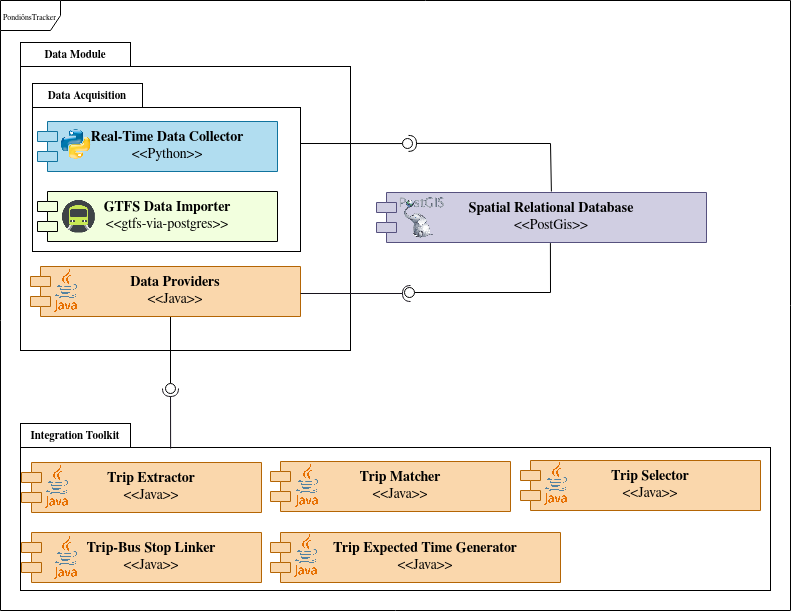
\includegraphics[width=.95\textwidth]{imagem/cap4/arq-pondionstracker.drawio.png}
        \source{The authors}
        \label{architecture:diagram}
\end{figure*}

{ \em Loose coupling} is the key design principle of \textit{PondiônsTracker} architecture to work with as many cities as possible, and this can be achieved by smaller software components that can be 
replaced or extended and still work with the other components with few adjustments, 
because the behaviors of the main components are defined in interfaces, so an object-oriented language as Java suits this scenario.
The major external dependency is the \textit{PostGIS}\footnote{Available at \url{https://postgis.net/}}
database, which provides spatial functions and stores the data.  


\section{Entities}
\begin{figure}[h]
     \centering
        \caption{Entities Class Diagram}
        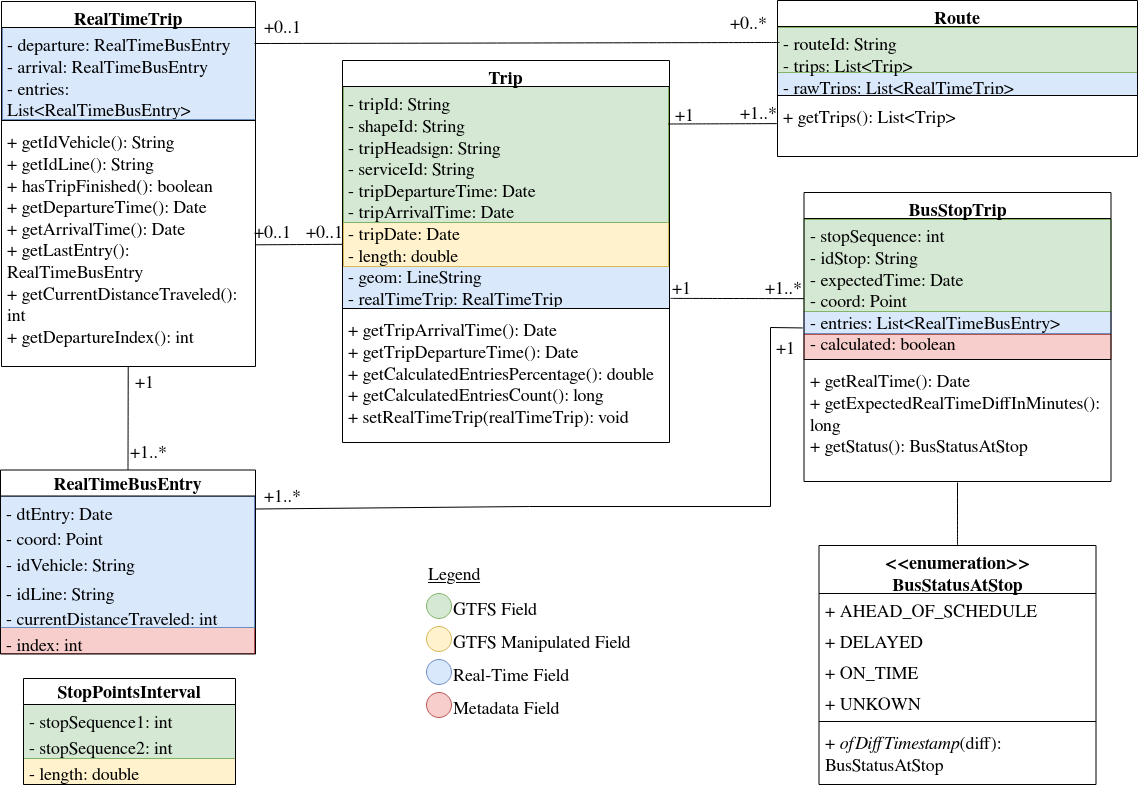
\includegraphics[width=\textwidth]{imagem/cap4/entitiesCD.png}
        \source{The authors}
        \label{cdEntities}
\end{figure}

In this Section, we present PondiônsTracker's entities used in all components, the entities
mix three types of fields: fields from the GTFS specification, fields to represent the 
real-time data and some auxiliary fields, Figure \ref{cdEntities} presents the entities 
class diagram with the getters and setters suppressed to improve the readability.
The fields highlighted in green are from the GTFS, and those highlighted in yellow are not originally from the given entity, but they are easily obtained by 
manipulating other fields, such as the \textit{Trip}'s $geom$ and \textit{BusStopTrip}'s
$coord$ which are spatial data from $shape\_id$, $stop\_lat$ and $stop\_lon$, respectively.
Finally, the fields highlighted in blue are from the real-time data,
and those highlighted in red were designed to store metadata produced during the components' execution.


The \textit{Route} and \textit{Trip} entities are defined at the GTFS specification, 
and we enriched both with more fields, the $rawTrips$ 
was added to the \textit{Route} to link with all the related raw 
real-time trips collected. Four new fields were introduced to the 
\textit{Trip}, two in yellow and two in blue, the yellow couple represents the spatial, 
in which $length$ represents the $geom$ length, that is a \textit{LineString} with
the bus stops are linked by the path programmed, in meters. Furthermore, in the blue couple,
$realTimeTrip$ corresponds to the real trip of a scheduled trip, which is a zero or one 
relationship, because
one $Trip$ can have at most one related \textit{RealTimeTrip}, but it also is unavailable, leading to a null reference. 
And $busStopSequece$ is a \textit{List} of all stops of this trip ordered by its $stop_sequence$, in other 
words, a list of \textit{BusStopTrip}.

The \textit{BusStopTrip} works as an entity that merges two GTFS's entities: \textit{stop\_times} and \textit{stops}. The first brings $stop\_sequence$, $stop\_id$, and $departure\_time$ that could be null
depending on the local GTFS. And, \textit{stops} provides the spatial information achieved 
using the $stop\_id$. The field $entries$, which is highlighted in blue, represents all the \textit{RealTimeBusEntry} related to this stop, which may be even zero, in other words, it is a
list containing every bus that was around this stop. Finally, the $calculated$ field in red
is a flag representing that this \textit{BusStopTrip} has no actual entry related to it, so an artificial 
entry was created and associated with this stop, as further explained in Section \ref{sub:integration}.
Finally, the method \textit{getStatus} gets the \textit{BusStatusAtStop} of the current \textit{BusStopTrip}, and this operation enables the delay analysis.

Then, for every bus positioning, around or not around a bus stop,
is entry from \textit{RealTimeBusEntry}, which is the entity that summarizes 
all \textit{PondiônsTracker}'s real-time required blue fields in a group of five as 
follows:
\begin{enumerate*}
    \item $dt\_entry$: Timestamp of the occurrence;
    \item $coord$: The location of the occurrence. Mainly given by lat/lon coordinates;
    \item $id\_vehicle$: A identifier for the vehicle executing the trip;
    \item $id\_line$: A identifier for the route/trip being executed;
    \item $current\_distance\_traveled$: The current distance traveled in a trip.
\end{enumerate*}
And a \textit{RealTimeTrip} is achieved by ordering the entries by its $dt\_entry$ 
then group them by $id\_vehicle$, which is the concept that a single bus can only travel
a single trip at a time. Finally, the field in red $index$ represents the position of an
entry in a trip.


\section{Data Module}
The Data Module's main goal is to encapsulate 
operations of the \textit{PostGIS} from the other components. 
There are three artifacts inside this module, 
\textit{DataImporter},
\textit{RealTimeDataCollector},
and \textit{DataProviders}, 
the first two components encapsulate writing, and the last encapsulate reading.
Also, there are two \textit{DataProviders}, one that works with GTFS data and the
other works with real-time data, \textit{GTFSProvider} and \textit{RealTimeProvider},
respectively.

\subsection{GTFS Data Importer}
The \textit{GTFS Data Importer} is a component that imports the GTFS data to the \textit{Postgis}
and creates the basic structure needed. So, given an instance of \textit{Postgis} running 
in a cloud service or local or dockerized environment, for instance, the first step is to 
execute the \ac{DDL} required, which is defined at \textit{schema.sql} that is a \ac{SQL} file 
located at $scripts/sql/$. 
\textit{schema.sql} defines two tables, and the first is called 
{\em  real\_time\_bus} is a table to store the real-time data. In other words, each row is
an instance of a \textit{RealTimeBusEntry}. And, for this table, there are two indexes,
one is over $dt\_entry$ and the other over $dt\_entry$ combined to $id\_vehicle$, 
they are designed to improve the performance of the queries executed by the \textit{Data Providers},
further explained in Subsection \ref{sub:dataProviders}. Figure \ref{fig:rmRTB} shows its relational model.

\begin{figure}[h]
\centering
\begin{minipage}[t]{.5\textwidth}
  \centering
  \caption{{\em  real\_time\_bus}'s \\relational model}
  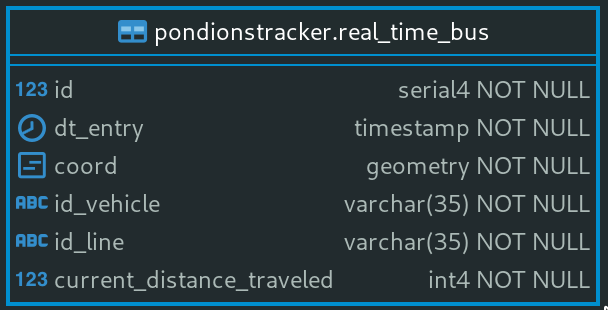
\includegraphics[width=.99\linewidth]{imagem/cap4/real_time_bus_ER.png}
  \source{The authors}
  \label{fig:rmRTB}
\end{minipage}%
\begin{minipage}[t]{.5\textwidth}
  \centering
  \caption{{\em  shapes\_summarized}'s \\relational model}
  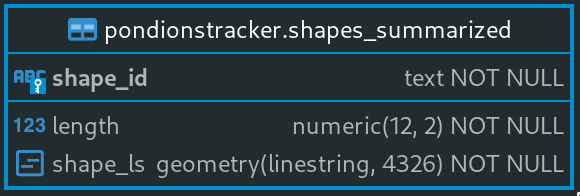
\includegraphics[width=.99\linewidth]{imagem/cap4/shapes_summarized_ER.png}
  \source{The authors}
  \label{fig:rmSS}
\end{minipage}
\end{figure}

Figure \ref{fig:rmSS} shows the relational model of the second table created, called {\em  shapes\_summarized} and is an auxiliary table 
that stores the geometric type $LineString$ and its length for all trips. 
This table is needed because the tool used to import the GTFS data does not
provide this structure or a similar one. The tool used is the \textit{gtfs-via-postgres} 
\footnote{Available at \url{https://github.com/public-transport/gtfs-via-postgres}},
an open-source solution to import static data that Google recommends. It takes as input the
GTFS files, which could be in the $.txt$ or $.csv$ format, and create a new table in the database for each
entity. 

Finally, the last step to fully initialize the database is to execute an SQL script that populates
the table {\em  shapes\_summarized}, which is \textit{shapes\_summarized\_populate.sql}
and it is located in the same folder as \textit{schema.sql}.
This SQL script takes the \textit{shapes} table grouped by the $shape\_id$
as input to the \textit{PostGIS}'s function { \em ST\_MakeLine} that produces a $LineString$ from the given points.

We provide a{ \em shell} script that executes all the steps described previously, this script is 
called $init.sh$, and it is in the folder $scripts$. This script takes two inputs: 
the first argument is the path to the folder where the GTFS's files are located, and 
the other argument is the schema name that \textit{gtfs-via-postgres} is going to import to.
$init.sh$ uses \textit{PostGIS}'s environment variables
\footnote{Available at \url{https://www.postgresql.org/docs/current/libpq-envars.html}}
to connect to the database, then execute three commands. The first loads \textit{schema.sql},
the second uses \textit{gtfs-via-postgres} to import the GTFS, and the third executes the 
\textit{shapes\_summarized\_populate.sql}.


\subsection{Real-Time Data Collector}
The \textit{Real-Time Data Collector} is the component responsible to 
collect the real-time data and insert it into {\em  bus\_real\_time},
encapsulating the writing into the database. In other words, this component will incorporate the data 
from real-time traffic \ac{API} provided by some external source into the table, such as traffic agencies.
Regarding extensibility, {\em bus\_real\_time} can be enriched with more data, 
instant speed, and direction, for instance.

The Real-Time Data Collector may be implemented in any language since
it must adapt to each real-case scenario to insert valid entries into the table
because it depends on the local city provider.
To illustrate a record, an API provides the following data:
A bus $b$ of line 123 is at a bus stop
near a drugstore and has already traveled 3 km on its route at 4 p.m.
The corresponding entry would be:
\begin{enumerate*}
  \item $dt\_entry$ as 16:00;
  \item $coord$ as the point composed by the latitude and longitude of the 
  bus stop near a drugstore where the $b$ is;
  \item $id\_vehicle$ as the $b$'s vehicle id;
  \item $id\_line$ as 123;
  \item $current\_distance\_traveled$ as 3000, which is 3km transformed to meters.
\end{enumerate*}
And the $id$ is generated and managed by the database.


\label{sub:dataProviders}
\subsection{Data Providers}

\begin{figure}[h]
     \centering
        \caption{Data Providers Class Diagram}
         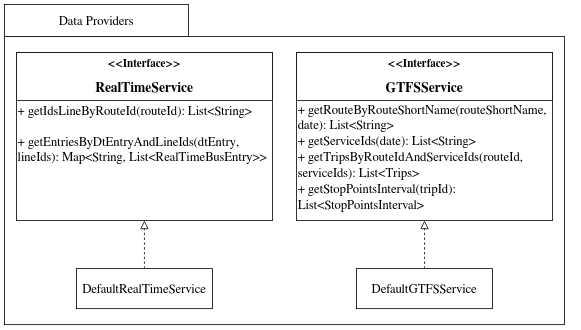
\includegraphics[width=.9 \textwidth]{imagem/cap4/dataProviderED.drawio.png}
        \source{The authors}
        \label{cdProviders}
\end{figure}

To isolate the access to the \textit{PostGIS}, the Data Providers are designed to 
supply all the data  required in other modules. Figure \ref{cdProviders} represents the class diagram for these components, then
it is composed of two interfaces: \textit{RealTimeService} and \textit{GTFSService}, which represent the real-time data 
and the GTFS data, respectively. 
Also, each of these interfaces has a default implementation, 
the \textit{RealTimeService} implementation is \textit{DefaultRealTimeService} 
and the \textit{GTFSService}'s default implementation is given by \textit{DefaultGTFSService}. 
The Data Providers are available at the Maven Repository and can be accessed by adding the 
following dependency to a \textit{pom.xml} in a Java 17+ project.
\begin{lstlisting}[language=XML]
		<dependency>
			<groupId>br.pondionstracker</groupId>
			<artifactId>data-module</artifactId>
			<version>1.0.0</version>
		</dependency>
\end{lstlisting}

The \textit{DefaultRealTimeService} implements the two methods defined by the interface. 
The first is called \textit{getIdsLineByRouteId}, It takes a route id
as input and produces a list containing all the line identifiers related to the given route, 
the default implementation is to return a list of a single item, which item is the inputted route id.
In other words, this method establishes the relationship between the two datasets heavily dependent
on each city context. Although this method is likely to be overridden, 
the default implementation assumes that the RT provider will use the $route\_id$.

The second method is called \textit{getEntriesByDtEntryAndLineIds}, it takes a target date and 
the $id\_line$s as input and produces a \textit{java.util.Map} whose key is $id\_vehicle$ and value
is a list of entries related to the $id\_vehicle$. So, the main idea, which is also implemented by the  
\textit{DefaultRealTimeService}, is to retrieve all the entries from a day of some lines ordered by $dt\_entry$ grouped by 
$id\_vehicle$, the \textit{TripExtractor} is going to take advantage of this grouping, 
as further approached in Subsection \ref{sub:2}.

The \textit{GTFSService}'s default implementation is given by \textit{DefaultGTFSService} 
which implements the four methods defined. The first is called \textit{getRouteByRouteShortName},
it takes a $route\_short\_name$ and a target date as input and produces a 
\textit{java.util.Optional} of a 
$Route$, the \textit{Optional} is going to be filled if the $route\_short\_name$ exists at the given date,
empty otherwise. The default implementation fills the $trips$ object using two other methods available,
\textit{getServiceIds} and \textit{getTripsByRouteIdAndServiceIds}. The method called \textit{getServiceIds}
takes a target date as input and retrieves all the valid $service\_id$s at the given date, that is, all the 
available services for that day of the week.

The method called \textit{getTripsByRouteIdAndServiceIds} takes a $route\_id$ and a \textit{List} of 
$service\_id$ as input and produces a \textit{List} of trips that is the schedule of each trip of that route. 
The default implementation retrieves the following fields: $trip\_id$, $shape\_id$, $service\_id$, 
$trip\_headsign$, $shape\_ls$, and $length$. Then, for each trip, the $busStopSequence$ is filled with
its stop sequence, stop id, expected time, and the bus stop coordinates. 
Finally, the last method is called \textit{getStopPointsInterval}, it takes a $trip\_id$ as input and 
produces a \textit{List} of \textit{StopPointsInterval}. That is, the trip's bus stops in sequence and
the distance between a couple of stops.



\section{Integration Module}
\label{sub:integration}
The Integration Module's main goal is to provide functions and methods to 
work with the transit data previously collected using the {\em GTFSService and RealTimeService}.
So, this module exposes seven interfaces, which are \textit{TripExtractor}, 
\textit{TripMatcher},
\textit{TripBusStopLinker},
\textit{TripSelector},
and \textit{TripExpectedTimeGenerator} as shown in Figure \ref{cdIntegration}. 
In the following Subsections, we get into details of the interface contracts
and its{ \em default} implementation. In the last Subsection, we approach the 
\textit{Drivers}. Finally, all the interfaces and their default implementation are  
available at the Maven Repository and can be accessed by adding the 
following dependency to a \textit{pom.xml} in a Java 17+ project.
\begin{lstlisting}[language=XML]
		<dependency>
			<groupId>br.pondionstracker</groupId>
			<artifactId>integration-module</artifactId>
			<version>1.0.0</version>
		</dependency>
\end{lstlisting}


\begin{figure}[t]
     \centering
        \caption{Integration Module Class Diagram}
        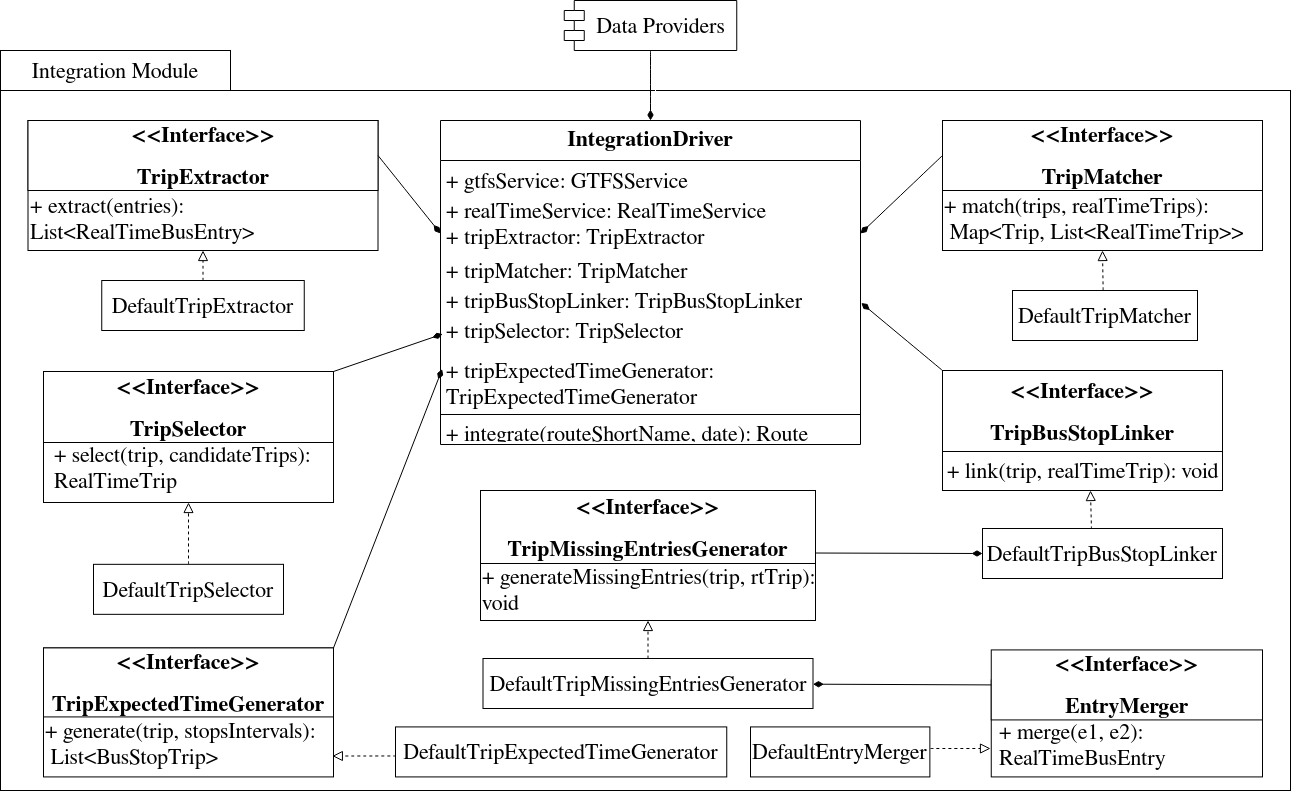
\includegraphics[width=\textwidth]{imagem/cap4/integrationModuleCD.png}
        \source{The authors}
        \label{cdIntegration}
\end{figure}


\subsection{Trip Extractor}
\label{sub:2}
The \textit{TripExtractor} is an interface that declares one method which is called
\textit{extract} that takes a \textit{List} of $RealTimeBusEntry$ as input and produces
a \textit{List} of $RealTimeTrip$. This component's main goal is to extract the trips from
entries because the data from the real-time API may not have a direct link to the GTFS, 
which leads to scenarios where APIs supply more data than the scheduled trips.
In other words, a trip represents a {\em trail} in the graph.
In addition, the APIs might return some unwanted trips, such as the displacement 
from the bus garage to a bus stop, and the other way around,
the{ \em default} implementation does not apply any strategy to filter out these 
trips. The implementation is defined in Algorithm \ref{alg:extract} and depends on three premises:
\begin{enumerate*}
    \item The entries must be from the same $idVehicle$;
    \item The entries must be sorted by $dtEntry$ in order to preserve their chronology;
    \item The $currentDistanceTraveled$ can only increase for the same trip.
\end{enumerate*}

After postulating these premises, it is iterated over entries, then for each entry,
it $currentDistanceTraveled$ is compared with a temporary variable $d$ defined on
line \ref{alg:extract:d}. If the entry's $currentDistanceTraveled$ is{ \em lower} 
than $d$, represented by the $if$ command on 
line \ref{alg:extract:if}, it implies that a trip has just finished due to the third premise at 
this point, it is assigned the $previousEntry$ to the $arrivalEntry$, on
line \ref{alg:extract:arrival}.
Otherwise, when $d$ is greater than or equal to the entry's 
$currentDistanceTraveled$ and the $arrivalEntry$ is still null, and the entry might be the $departureEntry$ or an intermediate entry.
Finally, after iterating over all entries, it is added to $trips$ the 
last trip that is composed of the variables $departureEntry$ and $previousEntry$,
the $previousEntry$ contains the{ \em last} entry of the List inputted, then 
$trips$ are returned.

\begin{algorithm}[t]
\caption{\textit{DefaultTripExtractor}'s implementation}\label{alg:extract}
\begin{algorithmic}[1]
\State $trips \gets [ ]$
\State $d \gets 0$ \Comment{currentDistanceTraveled}
 \label{alg:extract:d}
\State $departureEntry \gets null$
\State $arrivalEntry \gets null$
\State $previousEntry \gets null$
\For{$i\leq entries.length; i++$} 
    \State $entry \gets entries[i]$
    \If{$entry.currentDistanceTraveled\geq d$}
    \label{alg:extract:if}
        \If{$arrivalEntry \neq null$}
            \State $trips.add(new Trip(departureEntry, arrivalEntry))$
            \State reset temp vars to initial state
        \Else
            \State $d \gets entry.currentDistanceTraveled$
        \EndIf
        \If{$departureEntry$ is null}
            \State $departureEntry \gets entry$
        \EndIf
    \Else
        \State{$arrivalEntry \gets previousEntry$}
        \label{alg:extract:arrival}
        \State $d \gets entry.currentDistanceTraveled$
    \EndIf
    \State{$previousEntry \gets entry$}
\EndFor 
\State $trips.add(new Trip(departureEntry, previousEntry))$
\State return trips
\end{algorithmic}
\end{algorithm}

Algorithm \ref{alg:extract}'s output is all the trips delimited by its vehicles 
and timestamps, but they are not linked to a route yet. 
The complexity of this algorithm is $O(n)$, in which 
that $n$ corresponds to entries generated by a single bus in an interval, and it is necessary to iterate once over $n$ to delimit the trips.
Despite the $O(n)$ 
complexity, it is worth noticing that $n$ corresponds to entries produced by a single 
bus in an interval, then Algorithm \ref{alg:extract} {\em might} be executed over a hundred times
for a single day of observation, for instance.

\subsection{Trip Matcher}
The \textit{TripMatcher} is an interface that declares one method, which is called
\textit{match} that takes two \textit{Lists} as input, one of $Trip$ and the other
of $RealTimeTrip$. Then, it produces a \textit{Map} of all $RealTimeTrip$s related to a 
$Trip$. So, this component is responsible for linking the static to the real-time data,
the{ \em default} implementation tries to unify the scheduled block with the 
delimited trips from real-time data by comparing \textit{Trip}'s 
and \textit{RealTimeTrip}'s $departureTime$. 
To do so, the key idea is to iterate over all the trips
from $trips$, and for each scheduled trip, all real-time trips 
that $departureTime$ is within an interval $i$ is reserved to the block otherwise, it is discarded. 

This interval represents the trip's maximum initial shifting 
and is a required argument to instantiate \textit{DefaultTripMatcher}, which is 
used to initialize the final field, $maxTripInitialShifting$. 
That is a minute interval that works to mitigate minor deviations from
the schedule at the start of  a trip that is likely to happen due to real-time data 
unpredictability. 
Then, $maxTripInitialShifting$ works both for delayed and ahead-of-schedule lefts because 
it is taken into account in an absolute value, 
for instance, when $maxTripInitialShifting=5$ it matches a trip that is 5 minutes delayed or 5 minutes ahead of schedule. Finally, to exactly match on-time trips, $maxTripInitialShifting = 0$. 

\textit{DefaultTripMatcher}'s complexity is $O(rt)$, in which $r$ is the size of $trips$
and $t$ is the size of $realTimeTrips$. $r$ is constant because its source
is the GTFS data, and $t$'s size is unstable due to the real-time data, 
so $\Omega(n^2)$, or even lower when $r > t$.
Despite having the lowest complexity, lower than $\Omega(n^2)$, this scenario
is undesired because it represents that there are more scheduled trips than 
trips collected, which indicates some degree of information loss. 
When $r = t$, it represents the best-case scenario regarding information
recovery because there is the same number of scheduled trips and trips collected,
corresponding to a complexity of strictly at $\Omega(n^2)$. In most cases, $r < t$ is due to
the unwanted trips, then $\Theta(rt)$.


\subsection{Trip Selector}
The \textit{TripSelector} is an interface that declares one method, which is called
\textit{select} that takes a $Trip$ and \textit{List} of $RealTimeTrip$ as input 
and produces a \textit{List} of $RealTimeTrip$. This component's main goal is to
{\em select} the $RealTimeTrip$ trip that better fits the $Trip$.
The default implementation selects the $RealTimeTrip$, which has the latest 
$departureTime$ that fills the two following conditions:
\begin{enumerate}
    \item The last entries $dtEntry$ must be after the $departureTime$;
    \item The trip must have traveled at least a $tripMinPercentageTraveled$ percentage of the \textit{Trip}'s $length$.
\end{enumerate}

$tripMinPercentageTraveled$ is a required argument to instantiate 
\textit{DefaultTripSelector} and it represents the \textit{RealTimeTrip}'s minimum percentage traveled of the \textit{Trip}. In other words, it is a parameter that
defines the concept of a completed trip. \textit{DefaultTripSelector} has 
a complexity of $O(n)$ because it iterates over the candidate real-time trips
and selects the trip with the latest $departureTime$ that fills the preconditions defined above.

It is necessary to select the candidate trip because there are some unwanted trips, such as the displacement from the bus 
garage to a bus stop and the other way around. Among all trips, some
unfinished trips get distinguished by not going through all bus stops on a route
due to many factors, such as
\begin{enumerate*}
  \item Bus breaking down.
  \item The bus' communication system is malfunctioning.
  \item A bus' last entry recorded is still en route.
\end{enumerate*}

\subsection{Trip-Bus Stop Linker}
The \textit{TripBusStopLinker} is an interface that declares one void 
method which is called \textit{link} that takes a $Trip$ and a $RealTimeTrip$ as input
and fills each $entries$ set from $Trip$'s $busStopSequence$.
In other words, this component's main objective is to link 
a real-time trip to the bus stop from a scheduled trip,
which binds static data alongside real-time data. 
Although this component can be used alone,
and it was designed to work with the output of the previous component
to enrich the trips with some initial route information.
The default implementation assumes that the $RealTimeTrip$ have
been around every bus stop from their route. 

Furthermore, in the context of the default implementation, 
the entry is considered to be around the bus stop if it is {\em at} or
{\em near}. Matching the entry and the bus stops is not a simple task due to GPS position errors caused by the
lack of synchronization between the datasets. 
These errors are pretty common 
and well-expected, it is unlikely that the entry's $coord$ is exactly 
{\em at} the bus stop for many reasons, such as the bus broke or was simply too fast, and the dataset missed capturing the instant. 
These issues are reported in 
\citeonline{routableTimetableGTFS}, and 
we adopted their concept of a distance threshold between an entry and the bus stop for positioning, and from here, we are going to reference this threshold as $d_t$, so an entry 
within $d_t$ is considered {\em at} a bus stop. Figure \ref{img:4:3} illustrates an
entry within $d_t$, and Figure \ref{img:4:emptyset} shows a couple of entries, $e_1$ and $e_2$, which are not 
within $d_t$, for instance.


\begin{figure}[h]
     \centering
        \caption{Entries and $d_t$ representations}
        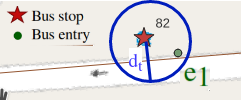
\includegraphics[scale=.65]{imagem/cap4/entriesDT.drawio.png}
        \source{The authors}
        \label{img:4:3}
\end{figure}

\begin{figure}[h]
     \centering
        \caption{Empty set of entries}
        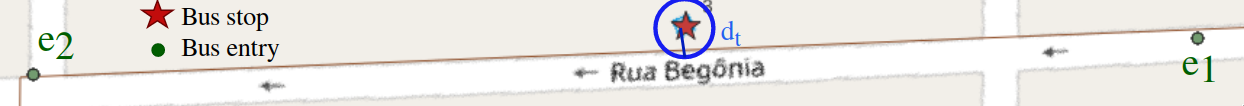
\includegraphics[width=\textwidth]{imagem/cap4/9202_empty_set.png}
        \source{The authors}
        \label{img:4:emptyset}
\end{figure}

So, the \textit{DefaultTripBusStopLinker} associates each bus stop from 
the scheduled trip with a set of entries there is within $d_t$.
However, an entry that is within $d_t$ is not necessarily 
part of the set because a single entry might be within $d_t$
of more than one bus stop. 
For instance, one avenue has a couple of bus stops on the same route
which are on opposite sides, and consequently, 
they are in different directions of the route. 
One entry between these two bus stops is related 
to only one of them, one bus cannot be at two stops simultaneously. Thus, the key idea is to match entries and bus
stops within $d_t$ and in the same direction as the route.

The default implementation key idea is to iterate over $Trip$'s $busStopSequence$
and for each bus stop $s_x$ it is searched for all the valid entries within $d_t$, then scanning the $RealTimeTrip$'s $entries$ set.
The three following premises are required to relate an entry $e$ to a bus stop $s_x$:
\begin{enumerate}
  \item an entry $e$ can be associated with only one $s_x$;
  \item a $s_x$ can be related to more than one entry $e$;
  \item a $s_x$ can be related to zero entries.
\end{enumerate}

The complexity of this operation is $O(n \log_k)$, in which
$n$ is the number of stops in a trip and $k$ is the size of entries of
the real-time trip. The first premise postulated assures the complexity of $\log_k$ when 
iterating through the entries set because the search for a stop $s_x$ starts at 
the index of the last entry related to a previous bus stop.

%\label{sub:generator}
%\subsection{Trip Missing Entries Generator: Entry Merger and Entry Merger Selector}

After executing the previous operation, each set of entries 
related to each bus stop should have {\em at least} one entry, 
but sometimes, the set is empty. 
And this does not imply that the bus has not been around a stop on the trip, 
it might be only a GPS positioning error. For example, if a bus is at a
certain speed, then it passes by a bus stop without stopping because there
are not any boarding nor landing at that given stop. Consequently, the
set of entries will be empty, and the third premise represents it. 
In other words, we know 
that the bus had been around to the stop, but there was not a single entry
close enough, as $e_2$ from Figure \ref{img:4:emptyset}. 
In this scenario, the \textit{DefaultTripBusStopLinker} executes an extra step
to generate an artificial entry at the stop with an empty set using the 
closest couple of entries, described by interface \textit{TripMissingEntriesGenerator}.

The \textit{DefaultTripMissingEntriesGenerator} design is to iterate over each 
bus stop $s_k$ from $Trip$'s $busStopSequence$ with no entry related to it. 
Then, each $s_k$
is going to be linked to a new artificial entry $e_g$ that is going to be
generated by the merge of a couple of entries. The \textit{EntryMerger} is the component
in charge of merging two entries, the strategy behind it is to execute a linear interpolation
between the two entries $coords$ and other attributes, which is a simple operation
whose complexity is \textit{constant}. To illustrate, if the merged entry $e_{(n-1, n)}$
is the product of $e_{n-1}$ and $e_n$ then it is going be as shown in Table \ref{tab:merger}.

\begin{table}[h]
\centering
\caption{Example of merge of $e_{n-1}$ and $e_n$ } 
\begin{tabular}{|l|c|c|c|c|}
\hline
\multicolumn{1}{|c|}{} & $dt\_entry$    & $coord$    & \multicolumn{1}{l|}{$id\_vehicle$} & \multicolumn{1}{l|}{$current\_distance\_traveled$} \\ \hline
$e_{n-1}$                & 10:00 &  coord $e_{n-1}$         & 1     &    5000     \\ \hline
$e_n$                & 10:02  & coord $e_{n}$ &               1    & 5100                   \\ \hline
$e_{(n-1, n)}$                & 10:01 & coord $e_{(n-1, n)}$ &    1               & 5050                 \\ \hline
\end{tabular}
\source{The authors}
\label{tab:merger}
\end{table}


The task of selecting which couple is going to be merged is complex as well and
it is performed by the interface \textit{EntryMergerSelector}.
For instance, given a bus stop $s_n$, in which $n$ represents the sequence of that stop on
the trip and $s_n$ has no entry related to it,
then an artificial entry $e_g$ is going to be generated by the merge of two other entries. 
In the default implementation,
the first step in choosing these entries to merge is to comprehend that one is before and 
another is after $s_n$ to guarantee that the bus had passed by the stop, and,
the fact that multiple entries may exist in between. 
So, the key idea is to search for the two closest entries to $s_n$
from an interval of entries ranging from a {\em Lower Bound Entry} 
and an {\em Upper Bound Entry}.


    \begin{figure}[h]
        \centering
        \caption{A more complex scenario of no entries within $d_t$}
        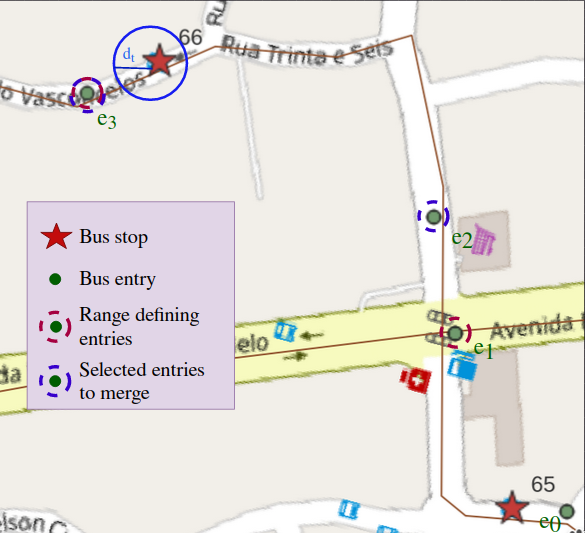
\includegraphics[scale=0.5]{imagem/cap4/9202_hard.png}
        \source{The authors}
        \label{img:4:4}
    \end{figure}

On the one hand, the {\em Lower Bound Entry} must be the entry with the latest $dt\_entry$
related to any other $s_{x}$ where $x < n$, that is the representation of 
the latest entry before $s_n$. On the other hand, the {\em Upper Bound Entry} 
must be the entry with the earliest $dt\_entry$ related 
to any other $s_{x}$ where $x > n$, which is the representation of 
the earliest entry after $s_n$. Figure \ref{img:4:emptyset} represents a scenario 
where the interval contains only the boundary entries so that they will be merged. Figure \ref{img:4:4} pictures a more complex scenario
in which to generate an entry related to the bus stop $S_{66}$ is needed to evaluate
the following set: $E = \{{e_1, e_2, e_3}\}$, then choose the two nodes with
the lowest distance to $S_{66}$, that are $e_2$ and $e_3$. In this case,
the {\em Lower Bound Entry} is $e_1$, and the {\em Upper Bound Entry} is $e_3$.

The \textit{DefaultTripMissingEntriesGenerator} complexity is $O(2n + c)$ because
the complexity of finding out each boundary entry is $O(n)$ and 
the merge algorithm adds the constant $c$. Then, the final complexity to 
generate an entry associated with a bus stop is $O(2n)$, consequently,
the \textit{DefaultTripBusStopLinker} complexity is $O(n \log n + 2n)$ which 
is the sum of the complexity of the two steps.




\subsection{Trip Expected Time Generator}
The \textit{TripExpectedTimeGenerator} is an interface that declares one method, which is called
\textit{generate} that takes a $Trip$ and \textit{List} of $StopPointsInterval$ as input 
and produces a \textit{List} of $BusStopTrip$, The default implementation generates the expected stop time using
the average route speed with the complexity of $O(n)$ where $n$ is
the number of stops. 

The \textit{DefaultTripExpectedTimeGenerator}'s key concept is that the stop times are incremental in the trip
and are incremented at each stop. In other words, for each bus stop, we increase to the initial $arrival\_time$ some time interval until the point it gets to the $departure\_time$ at the last bus stop. 
This time interval referenced is calculated for a bus stop 
$S_n$ using two values: 
the distance between $S_{n-1}$ and $S_n$ and the average trip speed.
The latter is constant due to the length of the trip and 
the required $arrival\_time$ and $departure\_time$ fields, which are used to infer the total
route duration, then the average trip speed is the division of the route length by the trip duration.

Calculating the distance between each $S_{n}$ and $S_{n+1}$ is not as straightforward as it looks
because of the route, the distance is not as simple as a line connecting these stops, and the paths
may contain turns and direction changes. An approach to this issue is the usage of 
Open Source Routing Machine's routing algorithms are similar to those used by \citeonline{routableTimetableGTFS} for map-matching. We relaid on the GTFS data, the {\em  shapes\_summarized} SQL table, 
and the following \textit{PostGIS} functions:
$ST\_LineLocatePoint()$, $ST\_Length()$ and $ST\_LineSubstring()$. 
Our approach consists of grouping and ordering the stops by couples using the $stop\_sequence$, 
consequently generating a route segment connecting each couple stop whose distance
is used to calculate the time needed to travel this segment.



Figure \ref{img:4:5} represents a bus stop couple for each record in which the first two 
columns indicate origin and destination stops, and the third and fourth columns are the 
linear distance and trip distance, respectively. For instance, the highlighted record
shows the route segment from bus stop 23 to 24, whose linear distance is around 400 meters
and the trip distance is 320 meters, so there is an 80-meter difference.


    \begin{figure}[h]
        \centering
        \caption{Example of bus stop couples and their distance}
        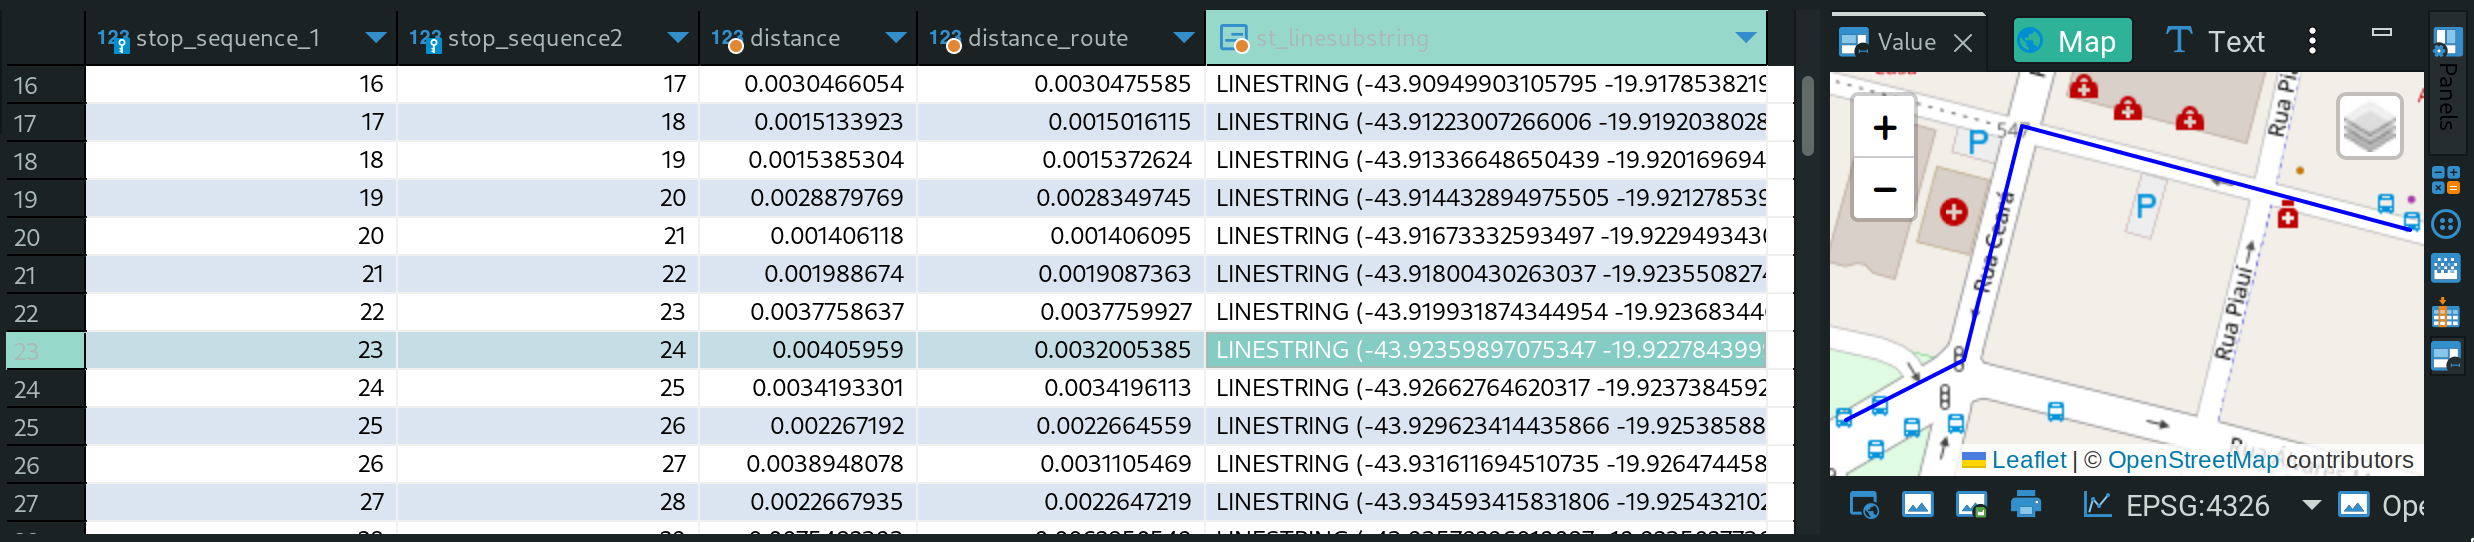
\includegraphics[width=\textwidth]{imagem/cap4/couplepoints.png}
        \source{The authors}
        \label{img:4:5}
    \end{figure}

Finally, given the building blocks, {\em Route Expected Time Generator} takes as input
routes information to calculate the average speed and route duration,
and a list of records such as Figure \ref{img:4:5}, which we iterate through leading 
to the complexity of $O(n)$. For each record, the route initial $arrival\_time$ is 
increased with the time needed to travel from a couple of bus stops at the average
speed of the route. In which {\em could} cause minor deviations to the original $departure\_time$ due to the precision 
of the calculus executed.



\subsection{Integration Driver}
The { \em Integration Driver} is the component that is composed, directly or indirectly, by the other components 
discussed in this Section to drive the execution from simple inputs as the $route\_short\_name$ and a target date
to produce a \textit{Route} instance completely filled. This component provides a default interaction not only 
between the \textit{Integration Module} components but also to the \textit{Data Providers} 
from the \textit{Data Module}.
Despite defining how the components interact, the { \em Integration Driver} depends on the abstraction
rather than the implementation, enabling the user to adapt the components to the particular scenario. Also,
it uses the default implementation with default values
for each component that is not overwritten by the user building a new instance.

    \begin{figure}[h]
        \centering
        \caption{Integration Driver Activity Diagram}
        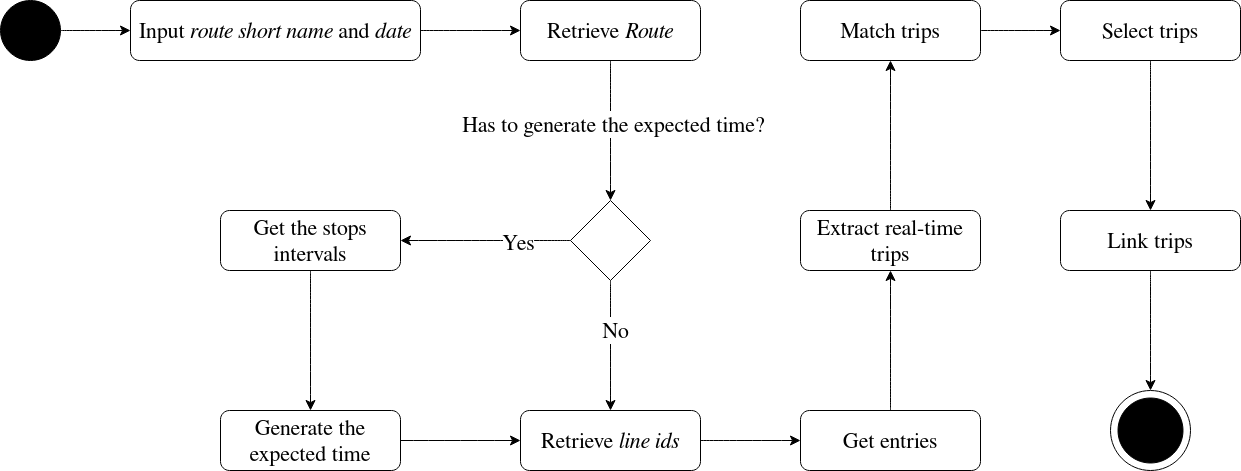
\includegraphics[width=\textwidth]{imagem/cap4/integrationDriverAD.drawio.png}
        \source{The authors}
        \label{img:4:integrationDriverAD}
    \end{figure}

Figure \ref{img:4:integrationDriverAD} shows the activity diagram of the \textit{integrate} method, which starts manipulating
the static data, then the real-time data, and finally, linking the two datasets. Also, Figure \ref{img:4:integrationDriverAD} 
also provides a high level point-of-view of the process to connect the datasets
.The first step
is to retrieve the \textit{Route} which is provided by the \textit{GTFSService} \textit{getRouteByRouteShortName}
method. Next, if the expected time at each bus stop for every \textit{Trips} of that
\textit{Route} is missing, then, before proceeding,
they are generated using the \textit{TripExpectedTimeGenerator}.
It takes the $stopsIntervals$ as input provided by the \textit{GTFSService} \textit{getStopPointsInterval} method. 
This scenario is due to the fact that the $arrival\_time$ and $departure\_time$ fields, from GTFS's $stop\_time$ 
\footnote{Available at \url{https://developers.google.com/transit/gtfs/reference#stop_timestxt}} entity is 
required just for the first and last stop of the trip.

After manipulating the static data, the next step starts by getting the $idsLines$ using the method 
\textit{getIdsLineByRouteId} from the \textit{RealTimeService}. Which is used as input to get all entries
from a day grouped by its $idVehicle$ using the method \textit{getEntriesByDtEntryAndLineIds}. In sequence, for each
vehicle, the trips are extracted in {\em parallel} using the \textit{TripExtractor}, then collected into a single
List, called $realtimeTrips$.

Finally, { \em Integration Driver} links the two datasets by matching the \textit{Route}'s \textit{Trips} 
with the real-time trips previously extracted using \textit{TripMatcher}'s \textit{match} method, that
uses a 5-minute interval, so $maxTripInitialShifting = 5$.
After matching,
it is required to select the most suitable real-time trip corresponding to a scheduled trip, which is executed by 
the \textit{TripSelector}, and the default implementation defines that a valid trip must have at least 85\% of its trajectory traveled. In other words, $tripMinPercentageTraveled = 0.85$. Then, the \textit{TripBusStopLinker}
links the bus stops with their respective entries for each scheduled trip with a real-time trip associated with,
the Driver defines a 50-meter range as the default value for $distanceThreshold$. Then, the \textit{Route} is returned.


\section{PondiônsTracker-BH}
In this Section, we present \textit{PondiônsTracker-BH}\footnote{Available at \url{https://github.com/Pongelupe/PondionsTracker-BH}} that is a \textit{PondiônsTracker}'s specialization created to
deal with Belo Horizonte's PTN particularities. So, we have implemented our own \textit{Real-Time Data collector}, and we have overwritten the method \textit{getIdsLineByRouteId} from the 
\textit{RealTimeService}.

\subsection{Real-Time Data Collector}
Belo Horizonte has a scenario similar to Rome's described in \citeonline{delays_bigdata}, in which  
different agencies provide the GTFS and real-time data. The GTFS is published
by the \textit{BHTrans}\footnote{Available at \url{https://dados.pbh.gov.br/dataset/gtfs-estatico-do-sistema-convencional}}, 
which is the local agency responsible for urban mobility planning. And 
the real-time data is provided by \textit{Transfacil}\footnote{Available at \url{https://dados.pbh.gov.br/dataset/tempo_real_onibus_-_coordenada}} which administrates the local bus services.
So, we developed our \textit{Real-Time Data Collector} in Python 3.11 to 
collect real-time data from Belo Horizonte's API.


\begin{table}[h]
\centering
\caption{Fields From The Real-Time API } 
\begin{tabular}{ |c|c|c|c| } 
\hline
Field name & Description & $real\_time\_bus$ related column \\
\hline
$EV$& Event code & - \\ 
\hline
$HR$& Timestamp & $dt\_entry$ \\ 
\hline
$LT$& WGS84 Latitude & $coord$ \\ 
\hline
$LG$& WGS84 Longitude & $coord$ \\ 
\hline
$NV$& Id vehicle & $id\_vehicle$ \\ 
\hline
$VL$& Instant speed & - \\ 
\hline
$NL$& Id line & $id\_line$ \\ 
\hline
$DG$& Vehicle's direction & - \\ 
\hline
$SV$& Trip way & - \\ 
\hline
$DT$& Distance displaced & $current\_distance\_traveled$ \\ 
\hline
\end{tabular}
\source{The authors}
\label{tab:entries-desc}
\end{table}

All entries collected were stored at $real\_time\_bus$ SQL table, but the API
has its own fields, which were translated to insert into the table. The API provides
nine fields. Table \ref{tab:entries-desc} describes each field and its translation to 
$real\_time\_bus$'s columns. 
Despite representing the $id\_line$ in the database, the $NL$ field 
is not a straightforward identifier to any GTFS entity, 
in other words, all bus entries retrieved from the API cannot be {\em directly} 
related to any trip or route. This scenario leads us to override  
\textit{RealTimeService}'s \textit{getIdsLineByRouteId} method, as further discussed
in the following Subsection.


\subsection{Belo Horizonte's \textit{RealTimeService}}
We created \textit{BHRealTimeService} to override \textit{getIdsLineByRouteId} method and use the default implementation for
the other methods, then \textit{BHRealTimeService} {\em extends} \textit{DefaultRealTimeService}. So, our implementation has to convert the
$route\_id$ using a \ac{CSV} conversion file
\footnote{Available at \url{https://dados.pbh.gov.br/dataset/tempo_real_onibus_-_coordenada/resource/150bddd0-9a2c-4731-ade9-54aa56717fb6}}
with 4 fields: $\_id$, $NumeroLinha$, $Linha$ e $Nome$. 

\begin{figure}[h]
     \centering
        \caption{Belo Horizonte's GTFS and RT data }
        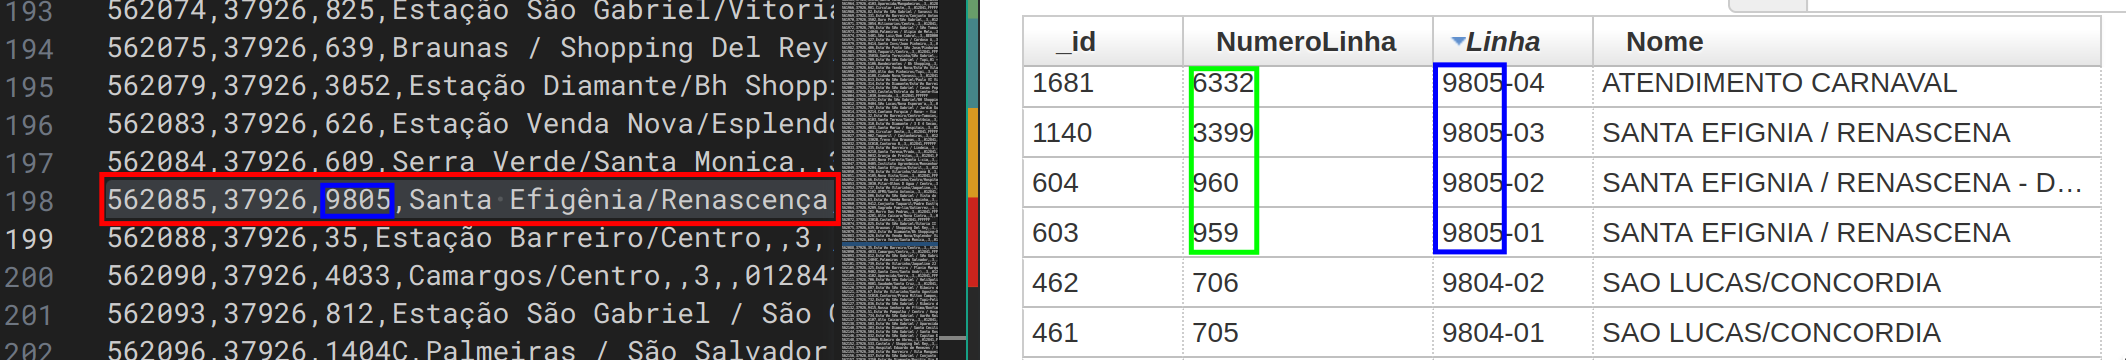
\includegraphics[width=\textwidth]{imagem/cap5/gtfsxapi.png}
        \source{The authors}
        \label{img:5:1}
\end{figure}

Figure \ref{img:5:1} shows Belo Horizontes's GTFS Routes on the left 
and the conversion table from the real-time data on the right. The first 
observation is that the column $NumeroLinha$'s domain is the $NL$, then 
$NumeroLinha = NL = id\_line$. The column $Linha$ resembles GTFS's $trip$ entity
and $routes$ relationship because it is also a \textit{one-to-many} relationship, 
in which a single bus line has multiple $Linha$ records.
For instance, the real-time API supplies an entry $e$ 
that its $NL$ is $959$, which value corresponds to an image from the domain of the 
column $NumeroLinha$ on the conversion table. Then, $959$ is going to be converted to 
$9805-01$, consequently $id\_route = 562085$.


To illustrate the \textit{one-to-many} relationship, in Figure \ref{img:5:1}
the route highlighted in red whose $route\_id$ is $562085$ has four related $NumeroLinha$ values, the group highlighted in green from the 
column $NumeroLinha$ on the conversion table. Because the group highlighted in blue
has the $route\_short\_name$ as the prefix. 
In this scenario, \textit{BHRealTimeService}'s \textit{getIdsLineByRouteId} is going
to return the group in green for $route\_id = 562085$, from the route highlighted in red.
